\documentclass[12pt]{article}
\usepackage{graphicx}
\usepackage{hyperref}
\usepackage{cite}


\begin{document}
\title{CSE441 Semester Project: FunCoin}
\author{Rob Kelly\\Sean Turner\\Randy Van Why}
\maketitle

\begin{abstract}
  The growth of public interest in cryptocurrencies in recent years has prompted the need for a simplified pedagogical model of the cryptocoin. ``FunCoin'' presents the cryptocurrency model in an easily understood way. FunCoin transactions are hashed to human-readable plaintext strings, and the FunCoin block header contains a readable list of transactions. Parameters for FunCoin mining can be adjusted to manually control difficulty. This allows interested users to experiment with possible applications of cryptocurrencies in a controlled setting.
\end{abstract}

\section{Introduction}
With the advent of global telecommunications and the internet in the past decade, methods of secure digital payments for goods and services have very quickly become an extremely important topic to a great many interested parties. One solution to the digital-commerce that has gained a great deal of traction quite recently is the idea of a cryptography-based ``cryptocurrency''. In just a few short years, cryptocurrencies have grown from an obscure topic of interest for cryptography enthusiasts and die-hard political activists to a widely-accepted payment solution in the online commerce marketplace. This growing trend of popular acceptance has spawned a growing crowd of cryptocurrency users interested in the possible applications of cryptocurrencies who may not be familiar with the underlying cryptographic principles on which popular cryptocurrencies are based.

What is needed is a new kind of cryptocurrency, designed not as a viable medium for financial transactions, but as a simplified model of cryptocurrency functionality that allows cryptocurrency enthusiasts to perform experiments on a small-scale in a controlled environment. Similar to Edward Schaefer's Simplified DES\cite{schaefer:sdes} encryption standard as a simplified analogue to DES, we present FunCoin as a simplified pedagogical model to cryptocurrencies like Bitcoin.

\section{Background}
In October of 2008, a white paper\cite{nakamoto:bitcoin} describing Bitcoin, a decentralized peer-to-peer electronic cash system, was published through cryptography mailing lists. While not the first attempt at an electronic payment-exchange system, Bitcoin was the first entry in the category of digital currencies known as ``cryptocurrencies'', which use concepts from cryptography and cryptographic protocols to secure transaction data. In the Bitcoin system, transactions are cryptographically-signed records of amounts with inputs and outputs -- an input to a transaction is signed to ensure it is only spent by its owner. Transactions are stored as leaves in a Merkle-tree block in the ``blockchain'', a public record of all blocks of all transactions. Bitcoins (also sometimes called ``satoshis'' after the author of the original paper) enter the economy as a reward for ``mining'', which involves finding an arbitrary bitstring nonce that, when combined with the header of the current block in the chain, can be hashed to a value less than some arbitrary difficulty limit. This scheme is called ``proof-of-work'', and is one of several possible block-timestamping solutions. While Bitcoin is the original and most popular cryptocurrency, several alternative cryptocurrencies have been established since, including Litecoin\cite{mcmillan:litecoin}, which uses \textsc{scrypt} instead of \textsc{SHA-256d} as a hashing algorithm, and Peercoin\cite{king:peercoin}, which uses proof-of-stake instead of proof-of-work as a block-timestamping scheme.

Initially, cryptocurrencies were used and promoted solely by cryptography enthusiasts\cite{slashdot:bitcoin} and those with a political interest in a decentralized currency. These early-adopters generally had a clear understanding of the fundamental concepts of cryptography that formed the basis of cryptocurrency protocols, but in more recent years the userbase for cryptocurrencies has expanded to include users who don't have the same background in cryptography. In just a few short years, the use of cryptocurrencies by the general public has grown at an impressive rate, and the effects of this growth are plainly outwardly-visible. The number of new transactions being added to the Bitcoin blockchain has grown from under 10,000 per day prior to 2012 to over 100,000 today\cite{blockchain:transactions}, and the Bitcoin mining hash rate has grown from about 20,000 Trillion hashes (GH/s) to over 300,000 GH/s in 2014 alone\cite{blockchain:hashrate}. The widespread use of cryptocurrencies has attracted the attention of government agencies\cite{irs:bitcoin}, as well.

\begin{figure}[h!]
  \centering
  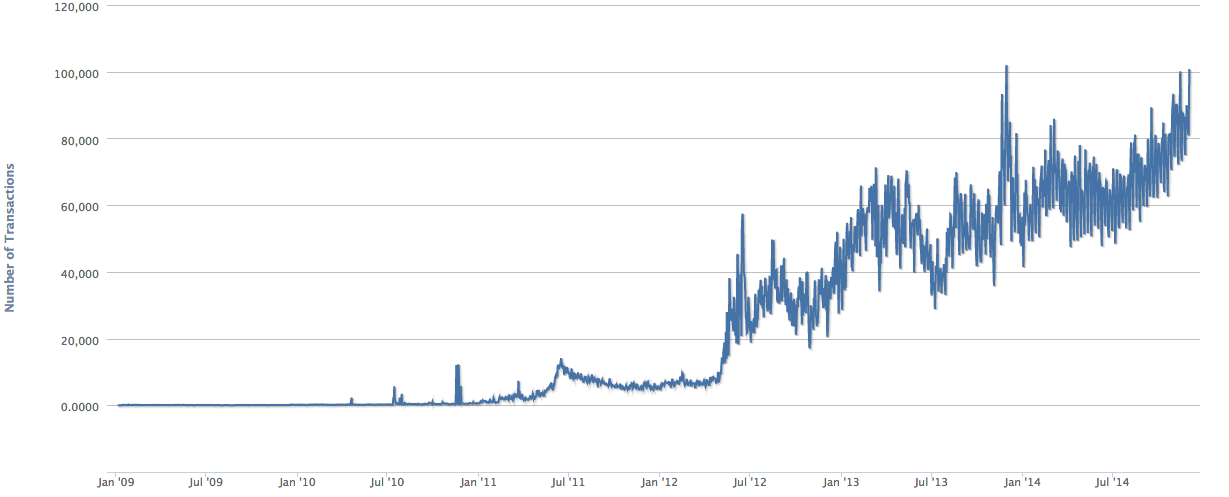
\includegraphics[width=\textwidth]{chart-transactions.png}
  \caption{Number of Bitcoin transactions made per day, 2009-present\cite{blockchain:transactions}}
\end{figure}
\begin{figure}[h!]
  \centering
  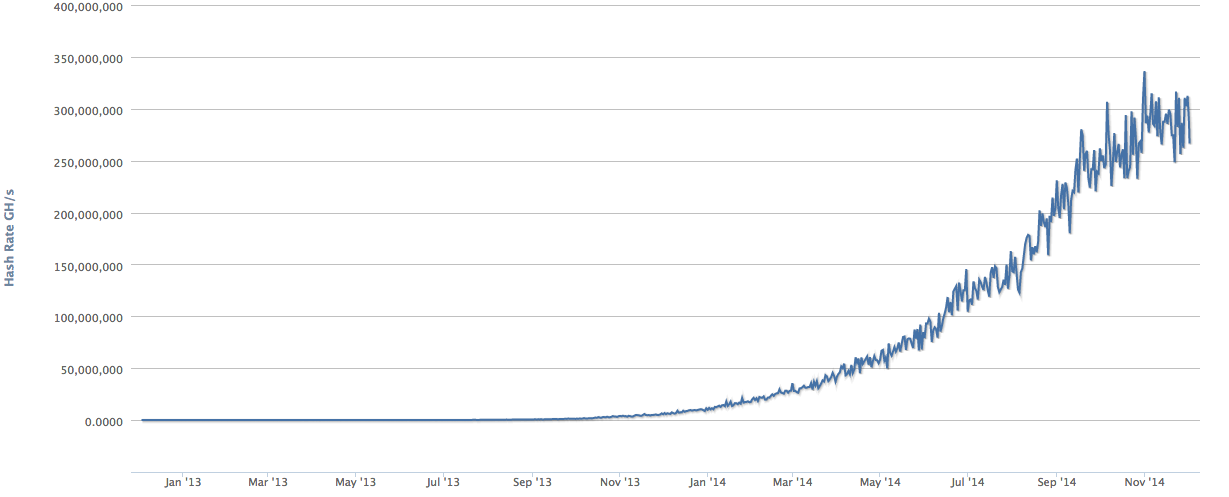
\includegraphics[width=\textwidth]{chart-hashrate.png}
  \caption{Bitcoin mining hash rate in GH/s, 2013-present\cite{blockchain:hashrate}}
\end{figure}

The unprecedented growth of Bitcoin has set off a chain-reaction in public interest in cryptocurrencies, and we expect this trend will only continue as Bitcoin starts to become accepted as a form of payment by more and more vendors\cite{chokun:vendors}. However, the complicated technical nature of the cryptographic foundations of cryptocurrencies as well as the structure and rationale of the protocol itself remain a major stumbling block to public understanding and acceptance of cryptocurrencies. 

\section{Approach}
\subsection{Motivation}
The goal of this project was to provide a pedagogical overview of cryptocurrencies on the whole
as well as attempt to discuss a theoretical implementation of a simple cryptocurrency for
demonstration purposes. In order to discuss our simplified model, the group took a look at
the most popular cryptocurrency implementation: Bitcoin.

\subsection{The BitCoin Implementation: An Overview}
The most natural starting point was for the group to think about the coin itself.
In Bitcoin-like cryptocurrencies, the coins that can be spent and mined are not
like traditional coins or electronic currency. Much of the implementation details
was clarified with the help of the Bitcoin paper\cite{nakamoto:bitcoin} and the
Bitcoin Developer Guide \cite{dev:guide}. 

\subsection{Transactions}
While it is obvious that Bitcoins are not physical coins, a surprising fact about
the currency is that Bitcoins are not even single digital entities or files at all.
Instead, Bitcoins are tracked and stored as transaction histories in a larger entity
known as the blockchain. An individual wishing to "spend" a Bitcoin simply signs
a hash of the transaction history and the receiver's public key using a digital signature
protocol. This is simply a cryptographically secure message that states that Party A agreed
to give the Bitcoin amount to Party B.

\begin{figure}[h!]
  \centering
  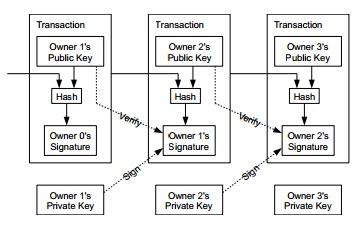
\includegraphics[scale=1]{transaction.png}
  \caption{Original Bitcoin transaction design \cite{nakamoto:bitcoin}}
\end{figure}

Thus the existence of the Bitcoin itself is governed solely by the transaction history. For our
simplified model we decided that each transaction would be a simple message indicating that Party
A has send $x$ amount of FunCoin to Party B. Thus a FunCoin transaction is a chain of such simple
messages. The authors realize that this approach is obviously not cryptographically secure. However,
the approach keeps to the main goal of design of a cryptocurrency that is easy to understand from an
outward perspective.

\subsection{Block Chain}\label{blockchain}
Figure \ref{figblockchain} (from the developer guide) sums up the basic structure of the blockchain nicely. 

\begin{figure}[h!]\label{figblockchain}
	\centering
	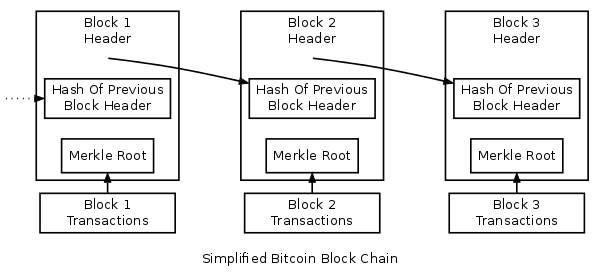
\includegraphics[scale=0.5]{en-blockchain-overview.png}
	\caption{Simplified block chain overview from \cite{dev:guide}}
\end{figure}

The blockchain constitutes the public ledger. It keeps transactions in order with timestamps and provides protection
against double spending. The heart of the blockchain is the Merkle tree. As can be seen in Figure \ref{figblockchain},
every block holds the root of this Merkle tree. This significantly improves the storage complexity of the blockchain since
the Merkle root is a small and easily transmitted piece of data that describes all the transactions in the block. And since
the block header already contains the hash of the previous block header, this gives us all the information we need about transactions. 

Our proposed simplified blockchain consists of a simplified Merkle tree-like tree structure sans the cryptographic hashing. Our
"transactions" are just human readable strings detailing where fundoshis went and how many.
This way, the "merkle root" can just be actually read, and the whole structure of the block chain is simple to understand.

\subsection{Verifying Coin Ownership}
Before Party B can accept payment, they must first verify that Party A has the Bitcoin to spend in the first
place. This is done by inspecting the blockchain. Party A sends Party B the pending transaction. Since every
transaction contains the history of all transactions leading up to it, Party B can check the blockchain
to ensure that the transaction history given is valid. Party B must check that the history
exists in the blockchain.

Bitcoin accomplishes validity via hashes. Party B will take the previous hash of all transactions before the pending one
and check to make sure that that hash exists in the blockchain. The actual Bitcoin implementation accomplishes
this in a space-saving manner via a merkel tree (see \ref{blockchain}).

%We may want to rethink this if we end up using a different design
Our simplified cryptocurrency would validate ownership by simply following the transaction history to the
genes of a single FunCoin. That would take care of local validity (to ensure the transaction is well formed).
From there, the receiver would check global validity by looking for the transaction history on the blockchain.

\subsection{Announcement of the Transaction}
From here, after the signature has occurred, the receiver announces the transaction to the rest of the network.
This announcement can be acheieved in different ways. In the Bitcoin protocol, the announcement is propagated throughout
the network with the goal of reaching as many network nodes as possible. In our simple protocol, we are assuming
that the pedagogical demonstrations will be small and thus transmitting the record of the transaction would be very trivial.

\subsubsection{Detecting Local Double-Spending Attacks}
Once a transaction has been announced, all nodes that "hear" the transaction save the transaction to the current block to
add to the blockchain. Any local double-spending attacks can be detected by checking the current block for a double spend.
Thus all nodes will reject any new transactions that attempt two different spends on the current block. This, however, does
not eliminate the possibility of a double spending (see \ref{doublespend}).

\subsection{Transaction Rounds}
Before a block is created and added to the blockchain, the Bitcoin protocol allows for a number of transactions to occur
during a time period. In the Bitcoin protocol, that time period is about 10 minutes (or the amount of time it takes to "mine"
the previous block \ref{mining}). 

\subsection{Double Spending and the 51\% Attack}\label{doublespend}

\section{Discussion}\label{future}
\subsection{Future Work}\label{work}
Some work that can be done to our implementation includes extending it from a simple client/server model to a true peer-to-peer cryptocurrency, making it more modular, so that interested parties may substitute their own implementations of key components such as the block chain and the proof of work in order to gain better understanding of the underlying techniques, and implement true transactions. 

Additional future projects include: implementing a wallet, considering different mining techniques altogether, and following on modularity, possibly making it into a library that can be used to roll your own simplified fun coin.

\subsection{Unsolved Problems}\label{unsolved}
Our biggest unsolved problem (and opportunity for Section \ref{future}) is to decentralize for a more accurate portrayal of how real cryptocurrencies function. Additionally, 

\bibliographystyle{abbrv}
\bibliography{report}

\end{document}
